\chapter{Artificial Neural Networks}
\label{ch:Artificial_Neural_Networks}

Artificial Neural Networks (ANNs) are computational systems which elaborate information likewise biological neural networks (animal brains).
These systems modify their behavior through a learning process and improve their accuracy in a certain task.
The underlying idea is that biological neural networks are superior in performance to computers and extremely more efficient in difficult tasks such as classification (e.g. image recognition) and prediction (e.g. pattern recognition).

Mathematically speaking, ANNs are a collection of nodes, each of them elaborate the information and is connected to the other in a certain amount.
Artificial networks can be either simulated on computers or physically built on specific hardware designed ad hoc.
At this time, ANNs are mainly implemented by simulations, however the technological progress is withheld by limitation in computing power and efficiency.
Training a complex artificial neural network with computers at the state of art might take even weeks.
Thus research on hardware architectures is surging: digital, analog, electrical, and optical devices are being developed.

This chapter is intended as an introduction to the world of artificial neural network, and focuses on the main aspects and types of neural networks, without claiming to be comprehensive.

\subsection{History}
\label{ssec:History}
It is widely acknowledged that the opening work of this research field was made in 1943 by Warren McCulloch and Walter Pitts, a neurophysiologist and a mathematician respectively.
In their research work, they described the operating mechanism of biological neurons by modeling a simple electronic circuit \cite{McCulloch1943}.

The following important work was made by Donald O. Hebb, who hypothesized the neural plasticity in 1949 \cite{hebb1949organization}.
He pointed out the fact that neural pathways are strengthened each time they are used, a concept known as \textit{Hebbian learning}.

During the late 1950s and the early 1960s, as computers became more powerful, many promising works were published.
Some simulated operation of artificial networks on calculators, e.g. Farley and Clark \cite{Farley1954} and Rochester \cite{Rochester1956}.
Other produced circuitry that implemented on hardware such networks, e.g. Rosenblatt \cite{frank1957perceptron,Rosenblatt1958}.
However, despite the early successes of neural networks, the traditional computing architecture (von Neumann architecture) was chosen as the preferred computing architecture.
As a result, funding and therefore also research diminished drastically in the following decades.

The reason this happened, probably, was due to several concurring facts.
First of all, in the same time period a research paper wrongly suggested that there could not be any multiple-layered neural network.
Moreover, the early successes of some works on neural networks pointed to an overestimation of the artificial neural networks potential, also held back by the technological capacity of the time.
Finally, important questions of philosophical nature come to light, such as the fear fueled debate on the impact on our society of a class of computers able to think.
This very controversy, i.e. artificial intelligence (AI) problem, is still a discussed topic today \cite{stanford.edu}.

Sometime during the 1980s the interest for this computing method was reinvigorated.
The main stimulation was probably given by a number of works which suggested methods to implement multi-layered networks distributing pattern recognition errors through the all the layers in the network.
This method is now called \textit{backpropagation}.

In today's research and technology, artificial neural networks are used in numerous applications.
However, the development is made slowly, due to technological limitation in computational power of present processors.

\subsection{Comparison with conventional computers}
\label{ssec:Comparison_with_conventional_computers}

%Digital, analog, and optical chips are the different types of chips being developed.
%One might immediately discount analog signals as a thing of the past.
%However neurons in the brain actually work more like analog signals than digital signals.
%While digital signals have two distinct states (1 or 0, on or off), analog signals vary between minimum and maximum values.
%It may be awhile, though, before optical chips can be used in commercial applications."

\section{Basis of Neural Networks}
\label{sec:Basis_of_Neural_Networks}

A neural network is a collection of processing elements, or nodes, interconnected in an arbitrary topology.
From its input nodes, the network accepts information, which will propagate into the inner nodes through the interconnections and will get elaborated at each node.
At the end of the network, there will be a number of output nodes, with the task of reading a portion of the inner nodes.
The inner nodes are also called hidden, because they are not meant to be accessible to the external world.
A generic scheme of such network is shown in \autoref{fig:generic_NN} \vpageref{fig:generic_NN}.

\begin{figure}[ht]
	\centering
	\tikzsetnextfilename{GenericNN}
\begin{tikzpicture}
	[%
	input/.style ={isosceles triangle,	draw=red!50,		fill=red!20,		thick,	inner sep=0pt,	minimum size=5mm},%
	inner/.style ={circle,							draw=black!50,	fill=black!20,	thick,	inner sep=0pt,	minimum size=5mm},%
	output/.style={rectangle,					draw=blue!50,	fill=blue!20,	thick,	inner sep=0pt,	minimum size=5mm},%
	]

	% nodes
	\foreach \i in {0,1,3} \node (input\i) at (0,2.5-\i) [input] {};
	
	\node (inner0) at (1.6, 0.2) [inner] {};
	\node (inner1) at (1.8, 2.0) [inner] {};
	\node (inner2) at (2.1, 1.2) [inner] {};
	\node (inner3) at (2.5,-0.6) [inner] {};
	\node (inner4) at (2.6, 3.0) [inner] {};

	\node (inner5) at (4.7,-0.2) [inner] {};	
	\node (inner6) at (5.0, 2.5) [inner] {};
	\node (inner7) at (5.3, 1.2) [inner] {};
	\node (inner8) at (6.0, 2.2) [inner] {};
	\node (inner9) at (6.2, 0.3) [inner] {};	
	
	\foreach \i in {0,1,3} \node (output\i) at (7.5,2.5-\i) [output] {};
	
	% interconnections
	\draw [->] (input0) to [out=0,in=180] (inner1);	
	\draw [->] (input0) to [out=0,in=180] (inner2);	
	\draw [->] (input0) to [out=0,in=180] (inner4);	
	\draw [->] (input1) to [out=0,in=180] (inner2);	
	\draw [->] (input1) to [out=0,in=180] (inner3);	
	\draw [dotted, ->] (0.5,0.5)  to [out=0,in=180] (inner0);	
	\draw [dotted, ->] (0.5,0.5)  to [out=0,in=180] (inner2);	
	\draw [->] (input3) to [out=0,in=180] (inner0);	
	\draw [->] (input3) to [out=0,in=180] (inner3);	
	
	\draw [->] (inner0) to (inner3);
	\draw [->] (inner0) to (inner2);
	\draw [->] (inner1) to (inner2);
	\draw [->] (inner1) to (inner4);
	
	\draw [dotted, ->] (inner2) to +(0:1);
	\draw [dotted, ->] (inner3) to +(0:1);
	\draw [dotted, ->] (inner4) to +(0:1);
	
	\draw [dotted, <-] (inner5) to +(180:1);
	\draw [dotted, <-] (inner6) to +(180:1);
	\draw [dotted, <-] (inner7) to +(180:1);
	
	\draw [->] (inner5) to (inner9);	
	\draw [->] (inner6) to (inner8);
	\draw [->] (inner7) to (inner8);
	\draw [->] (inner7) to (inner9);
	
	\draw [->] (inner5) to [out=0,in=180] (output3);
	\draw [->] (inner7) to [out=0,in=180] (output1);
%	\draw [dotted,->] (inner7) to [out=0,in=180] (7.25,0.5);	
	\draw [->] (inner8) to [out=0,in=180] (output0);
%	\draw [->] (inner8) to [out=0,in=180] (output1);
	\draw [dotted,->] (inner9) to [out=0,in=180] (7.25,0.5);	
%	\draw [->] (inner9) to [out=0,in=180] (output3);
	
	\foreach \i in {0,7.5} \node at (\i,0.6) {$\vdots$};
	
\end{tikzpicture}
	\caption{	Generic scheme of a neural network. %
						Triangles (red) are input nodes, circles (grey) are inner nodes, and squares (blue) are output nodes. %
						Interconnections among nodes are represented by arrows: %
						continuous when both elements are drawn, and dotted otherwise. %
						I chose a non-standard representation to emphasize the nonlinear nodes, which will use a nonlinear activation function. %
						}
	\label{fig:generic_NN}
\end{figure}

Each node can operate in the same way of the others or in a completely different manner, depending on the type of neural network.
The operation of nodes resembles that of animal neurons: various input gets collected and elaborated together to obtain an output, which will become one of the many inputs for subsequent neurons/nodes.
Specifically, the most used model for neurons is the McCulloch–Pitts (MCP) neuron.
It is divided into two parts, as shown in \autoref{fig:generic_node} \vpageref{fig:generic_node}: the first part is a weighted sum of the inputs, while the second part is given by the so called activation function.

\begin{figure}[ht]
	\centering
	\tikzsetnextfilename{GenericNode}
\begin{tikzpicture}
	\node [shape=circle, minimum size=2cm, draw=gray!100, fill=gray!20]%
				(af) at (1.5,0) {\LARGE $f_a$};
	\node at (af.south) [below, align=center] {activation \\ function};
	\node [regular polygon, regular polygon sides=6, minimum size=2cm, draw=gray!100, fill=gray!20]%
				(ws) at (-2,0) {\LARGE $\Sigma$};
	\node at (ws.south) [below, align=center] {weighted \\ sum};
	\draw (ws) to (af);
	\foreach \i in {1,2,4}	\draw (-4.5,1.5-0.6*\i) .. controls (-3.5,1.5-0.6*\i) .. (ws);
	\draw [dashed] (-4.5,-0.3) node {$\vdots\qquad$} .. controls (-3.5,-0.3) .. (ws);
	\foreach \i in {1,2}		\node at (-4.5,1.5-0.6*\i) [left] {$x_\i$};
	\node at (-4.5,-0.9)  [left] {$x_n$};
	\draw (-2,1.5) node [above] {$w_0$} to (ws);
	\draw (af) to (3.5,0) node [right] {$y$};
\end{tikzpicture}
	\caption{Generic node representation. $x$-values are inputs, $y$-values are outputs, $w_0$ is the bias.}
	\label{fig:generic_node}
\end{figure}
The node is described mathematically by \autoref{eq:Generic_node_function}
\begin{equation}
y = f_a \left(  w_0 + \sum_{i=1}^{n} w_i x_i \right),
\label{eq:Generic_node_function}
\end{equation}
where $f_a$ is the activations function, evaluated on the sum of the input $x_i$ weighted with $w_i$, plus a bias $w_0$.

Each node accepts values at its inputs and produces an output accordingly.
However, the output depends also on the node's parameters: the weights and the bias, which are usually changed outside the operative phase of the neural network, as I will explain in \autoref{sec:Working_Principles_of_ANNs} later \vpageref{sec:Working_Principles_of_ANNs}.

Moreover it is mandatory for the activation function $f_a\left(\cdot\right)$ to be nonlinear, because otherwise a collection of nodes will result in just a weighted sum of its inputs.
Two examples of nonlinear function are shown below in \autoref{fig:activation_function_examples}.

\begin{figure}[ht]
	\begin{subfigure}[b]{0.49\textwidth}
		\centering
		\tikzsetexternalprefix{tikz/}	% set subfolder
\tikzsetnextfilename{HeavisideThetaFunction}
\begin{tikzpicture}[baseline]
	\begin{axis}[%
%			yticklabel pos=upper,%
			title ={$\Theta(x)$},%
			xlabel={$x$},%
%			ylabel={$\Theta(x)$},%
		]
		\newcommand\LIM{5}
		\addplot [blue, domain=-\LIM:0,	samples=501,]	{0};
		\addplot [blue, domain=0:\LIM,		samples=501,]	{1};
	\end{axis}
\end{tikzpicture}
		\caption{}
		\label{fig:activation_function_example_1}
  \end{subfigure}
  \begin{subfigure}[b]{0.49\textwidth}
  		\centering
		\tikzsetexternalprefix{tikz/}	% set subfolder
\tikzsetnextfilename{LogisticFunction}
\begin{tikzpicture}[baseline]
	\begin{axis}[%
%			yticklabel pos=upper,%
			title ={$\mathrm{Logistic}(x)$},%
			xlabel={$x$},%
%			ylabel={$\mathrm{Logistic}(x)$},%
			thick,
			samples=101,
			smooth
		]
		\newcommand\LIM{10}
		\addplot [cyan, 		domain=-\LIM:\LIM]	{(1+exp(-0.5*x))^-1};
		\addplot [blue,	 	domain=-\LIM:\LIM]	{(1+exp(-1.0*x))^-1};
		\addplot [magenta,	domain=-\LIM:\LIM]	{(1+exp(-2.0*x))^-1};
		\addplot [red, 		domain=-\LIM:\LIM]	{(1+exp(-5.0*x))^-1};
	\end{axis}
\end{tikzpicture}
		\caption{}
		\label{fig:activation_function_example_2}
  \end{subfigure}
  \caption{Examples of activation function: (\ref{fig:activation_function_example_1}) is the well-known step function, or Heaviside $\Theta$, (\ref{fig:activation_function_example_2}) depicts a few functions from the family of the Logistic functions.}
  	\label{fig:activation_function_examples}
\end{figure}

One can distinguish at least three type of nodes in every neural network: input, inner/hidden, and output nodes.
Input nodes take one input value, from the outside of the neural network, and pass it on to the inner nodes unchanged.
Inner/hidden nodes take many inputs and generate an output through the activation function.
Output nodes, similarly to input nodes, take one input value, from the inside of the NN, and pass it on to the outside.

%This is not the orthodox description, but I claim that it is more consistent than the standard representation with the idea of functional \textit{black box}, in which input and output are the only visible nodes, while the other are hidden inside.
This is not the orthodox description, however it is consistent with the idea of functional \textit{black box}, in which input and output are the only visible nodes, while the other are hidden inside.
Therefore I can easily distinguish the nodes which will use a nonlinear activation function.
%Questa non è la visione standard/ortodossa, ma è consistente con un'idea di 'black box' in cui gli input e output sono gli unici nodi visibili. mentre gli altri sono all'interno della scatola nera.

\begin{figure}[ht]
	\centering
%	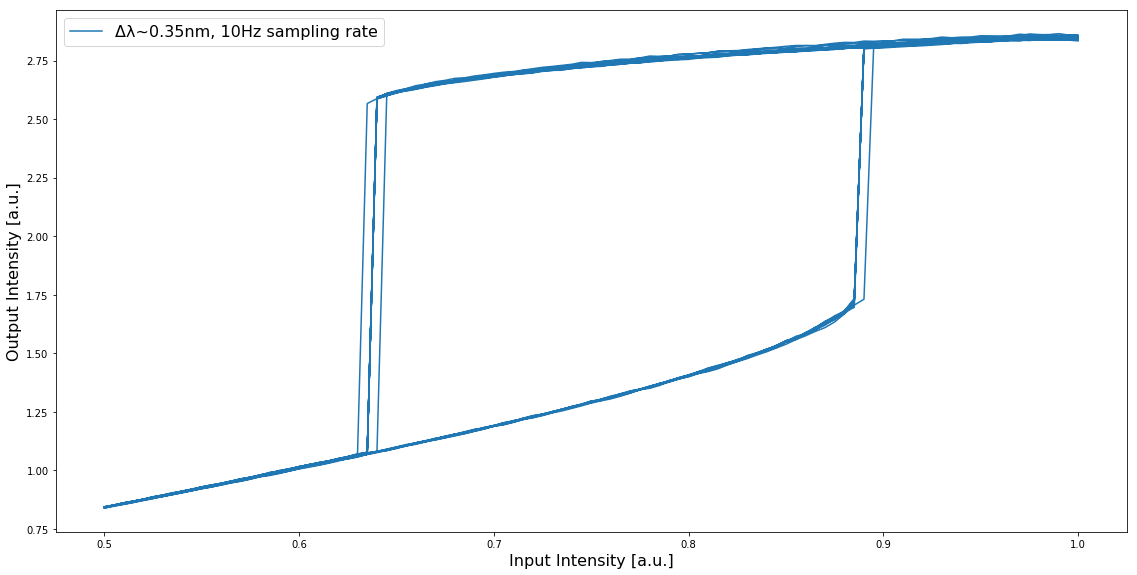
\includegraphics[draft,width=9cm,height=6cm]{figures/foo.png}
	\tikzsetnextfilename{BlackBoxNN}
\begin{tikzpicture}
	[%
	input/.style ={isosceles triangle,	draw=red!50,		fill=red!20,		thick,	inner sep=0pt,	minimum size=5mm},%
	inner/.style ={circle,							draw=black!50,	fill=black!20,	thick,	inner sep=0pt,	minimum size=5mm},%
	output/.style={rectangle,					draw=blue!50,	fill=blue!20,	thick,	inner sep=0pt,	minimum size=5mm},%
	]

	\newcommand\lin{0}
	\newcommand{\lout}{5}
	
	% black box
	\filldraw [thick, draw=black, fill=gray!90, line width=0.5mm] (0.1,-1.5) rectangle (4.9,3.5);	
	
	% nodes
	\foreach \i in {0,1,3} \node (input\i) at (\lin,2.5-\i) [input] {};
	
	\foreach \i in {0,1,2,4} \node (output\i) at (\lout,3-\i) [output] {};
	
	\node (inner0) at (1.6, 0.2) [inner] {};
	\node (inner1) at (1.8, 2.0) [inner] {};
	\node (inner2) at (2.1, 1.2) [inner] {};
	\node (inner3) at (2.5,-0.8) [inner] {};
	\node (inner4) at (2.6, 3.0) [inner] {};

	\node (inner5) at (2.8,-0.1) [inner] {};
	\node (inner6) at (3.0, 2.3) [inner] {};
	\node (inner7) at (3.3, 1.2) [inner] {};
	\node (inner8) at (3.9, 2.1) [inner] {};
	\node (inner9) at (4.0, 0.0) [inner] {};
	
	\node (input2)		at (\lin,0.5) {}; 		\node at (\lin,0.6) {$\vdots$};
	\node (output3)	at (\lout,0.0) {}; 	\node at (\lout,0.1) {$\vdots$};
	
	% interconnections
	\draw [->] (input0) to [out=0,in=180] (inner1);
	\draw [->] (input0) to [out=0,in=180] (inner2);
	\draw [->] (input0) to [out=0,in=180] (inner4);
	\draw [->] (input1) to [out=0,in=180] (inner2);
	\draw [->] (input1) to [out=0,in=180] (inner3);
	\draw [->] (input1) to [out=0,in=180] (inner4);
	\draw [dotted, ->] (0.5,0.5)  to [out=0,in=180] (inner0);
	\draw [dotted, ->] (0.5,0.5)  to [out=0,in=180] (inner1);
	\draw [dotted, ->] (0.5,0.5)  to [out=0,in=180] (inner2);
	\draw [->] (input3) to [out=0,in=180] (inner0);
	\draw [->] (input3) to [out=0,in=180] (inner3);
	
	\draw [->] (inner0) to (inner3);
	\draw [->] (inner0) to (inner5);
	\draw [->] (inner1) to (inner4);
	\draw [->] (inner1) to (inner6);
	\draw [->] (inner1) to (inner7);
	\draw [->] (inner2) to (inner5);
	\draw [->] (inner2) to (inner6);
	\draw [->] (inner2) to (inner7);
	\draw [->] (inner3) to (inner9);
	\draw [->] (inner4) to (inner6);
	\draw [->] (inner5) to (inner7);
	\draw [->] (inner5) to (inner9);
	\draw [->] (inner6) to (inner7);
	\draw [->] (inner6) to (inner8);
	\draw [->] (inner7) to (inner8);
	\draw [->] (inner7) to (inner9);
	
	\draw [->] (inner4)  to [out=0,in=180] (output0);
	\draw [->] (inner8)  to [out=0,in=180] (output1);
	\draw [->] (inner7)  to [out=0,in=180] (output2);
	\draw [dotted, ->] (inner9)  to [out=0,in=180] (output3);
	\draw [->] (inner3)  to [out=0,in=180] (output4);
	
\end{tikzpicture}
	\caption{Representation of the black-box concept}
	\label{fig:black_box_NN}
\end{figure}

%A neural network is an interconnected assembly of simple processing elements, units or nodes, whose functionality is loosely based on the animal neuron. The processing ability of the network is stored in the interunit connection strengths, or weights, obtained by a process of adaptation to, or learning from, a set of training patterns.

\noindent\uppercase{\large{What are neural network good for?\\ when do i talk about that?\\ e.g. NN are good for pattern recognition.}}
\normalsize

\section{Working Principles of ANNs}
\label{sec:Working_Principles_of_ANNs}
Because of its topology, each neural network will behave in a different manner from other neural networks with diverse, or even similar, arrangements of nodes.
Moreover the same neural network will perform a certain task better or worse also depending on how inputs are weighted at each hidden node, and normally those parameters are initialized with a random value at the creation of the network.
For this reason, before a neural network is considered ready to perform a task, it usually must go through three training stages: learning phase, validation phase, and testing phase.
Every one of these stages is meant to prepare the network to work as required from the designer.

\subsection{Learning Process}
\label{ssec:Learning_Process}
During the learning process the neural network is run on a set of known inputs $x$, each paired with its correct answer $y$, or target, in a second set of data.
The neural network will produce at the output a third set $\hat{y}$, which should be as close as possible to the correct answers, when the network works properly.
However this happens rarely, if ever, and a change in the way data is elaborated becomes necessary.
The usual \ref{} way is to keep the same topology, but tweak the weights that connect the hidden nodes together.
On account of this need, one needs to quantify the distance of the predicted result of the artificial neural network from the correct answer.
This is made by means of the loss function.

\subsubsection{Loss function}
\label{sssec:Loss_function}
The loss function $L(y, \hat{y})$ evaluates the difference between the predicted and the correct answer.
Usually, this quantity is linked to the geometrical distance between the predicted output and the target $\left| \hat{y}-y \right|$.
The most common loss function is the \textit{mean-square error}.
Assuming to have an input set of $N$ examples paired with the same number of targets, and that the outputs and the targets are composed by $C$ values, or classes, the function becomes:
\begin{equation}
	L(y, \hat{y}) = f_{MSE}(y, \hat{y}) = \frac{1}{N} \sum_{n=1}^N \sum_{i=1}^C \left( \hat{y}_{n,i} - y_{n,i} \right)^2,
\end{equation}
where each example in the set is subtracted to its target and then squared.
Finally the mean of all squares gives the expected result.

Another commonly used function is the cross-entropy loss (also known as negative log likelihood),
\begin{equation}
	L(y, \hat{y}) = f_{CEL}(y, \hat{y}) = - \frac{1}{N} \sum_{n=1}^N \sum_{i=1}^C y_{n,i} \log \left( \hat{y}_{n,i} \right),
\end{equation}
which expects positive values at the input.
Hence the error $-y\log \left( \hat{y} \right)$, quantified for each element in each example, is always a positive number.
The mean over all examples in the set returns the results.

Alternatively, variations of the previous methods are given by not taking the sum of the examples in place of the mean, or by calculating a loss function for each example instead of evaluating it for the whole set.

\subsubsection{Weights Update Process}
\label{sssec:Weights_Update_Process}

The weights update process is a difficult task, and probably the most computationally expensive one in running a neural network.
There is a variety of methods to chose from, depending on the type of artificial network and the resources available.

A widely used algorithm is the gradient descent, from its most simple version to more complex variations such as stochastic gradient descent (SGD).
This method updates the weights by subtracting a value proportional to the gradient of the loss function in respect to the weights themselves times a positive factor called \textit{learning rate}, as shown below.
\begin{equation}
	\left.w_i\right|_{n+1} = \left.w_i\right|_n - lr \cdot \frac{\partial L}{\partial \left.w_i\right|_n}
\end{equation}
where $\left.w_i\right|_{n}$ are the current weights, $lr$ is the learning rate, $\dfrac{\partial L}{\partial \left.w_i\right|_n}$ is the first derivative of the loss function in respect to the i-th weight at the current step, and $\left.w_i\right|_{n+1}$ are the updated weights.
%Hence it is necessary to calculate the gradient $\bigtriangledown_w L$.
This method is equivalent to minimize the error on the loss function, by following the gradient $\bigtriangledown_w L$.
This vector lives in the multidimensional space of the loss function $L:\mathbb{R}^W \mapsto \mathbb{R}$, where $W$ is the total number of parameters in the network.

The most efficient \ref{} algorithm is called \textit{backpropagation}: it computes the first derivative of the loss function $L$ in respect to all the parameters of the network, the weights, starting from the end of the artificial network and going backward toward the input, hence the name backpropagation.
Since the number of connections between nodes might be even order of magnitude bigger than the number of nodes, it is simple to understand how large networks are computationally expensive to train.

\paragraph{Other types of learning processes} are used, e.g. unsupervised/reinforced.

\subsection{Validation Process}
\label{ssec:Validation_Process}

\subsection{Testing Process}
\label{ssec:Testing_Process}
At the end, there is the process of testing the artificial neural network.
Ideally the network is tested on a new set of data, for which the target results are known, similarly to the preceding phases.
This time, however, the predicted outputs are compared to the correct answers to obtain an overall value for the correctness, often expressed in percentage.

\subsection{Datasets}
\label{ssec:Datasets}
Since there are three phases of preparation for any artificial neural network, there must be an appropriate number of examples to feed to it.

\noindent\uppercase{\normalsize{how do i divide a dataset?\\ what happens when there are too few examples?\\ And when there are too many?}}
\normalsize

\section{Feedforward NN}
\label{sec:Feedforward_NN}

The first and most simple type of neural network is called Feedforward.
In this kind of neural network, nodes are divided into groups called \textit{layers}.
A layer is a collection of nodes that accepts inputs from a preceding group and generate as many outputs as the number of nodes in the layer.
Each layer of a Feedforward neural network is connected in series with the others, except of input layer at the beginning and the output layer at the end.
As for the single nodes, the inner layer are called hidden, because usually not accessible.

The information travels from the input to the output and gets elaborated from each hidden layer: there are no connection between nodes of the same layer, nor loops or feedback between layers.
Depending on the topology of the network, there might be more or less layers, each composed by the same or a different number of nodes.
Moreover the connection between the layers might be complete, i.e. each node in the layer accepts each input of the preceding layer, in that case the layer is said to be \textit{fully connected}, or sparse as in the case of convolutional layers (see \autoref{par:Convolutional}).

\subsubsection{Perceptron}
\label{sssec:Perceptron}

The most naive topology of a Feedforward neural network is given by the so called \textit{Perceptron}.
The Perceptron dates back to the 1957, when the homonym \textit{Perceptron algorithm} was software implemented by Frank Rosenblatt on a computer (IBM 704) and only subsequently in hardware as the \textit{Mark 1 perceptron}\cite{frank1957perceptron,Rosenblatt1958}.
The graph of a generic (single layer) perceptron ANN is shown in \autoref{fig:Perceptron} below.

\begin{figure}[ht]
	\centering
	\tikzsetnextfilename{PerceptronNN}
\begin{tikzpicture}
	[%
	input/.style ={isosceles triangle,	draw=red!50,		fill=red!20,		thick,	inner sep=0pt,	minimum size=5mm},%
	inner/.style ={circle,							draw=black!50,	fill=black!20,	thick,	inner sep=0pt,	minimum size=5mm},%
	output/.style={rectangle,					draw=blue!50,	fill=blue!20,	thick,	inner sep=0pt,	minimum size=5mm},%
	]

	\newcommand\lin{0}
	\newcommand{\lhid}{3}
	\newcommand{\lout}{5}
	
	% nodes
	\foreach \i in {0,1,3} \node (input\i) at (\lin,2.5-\i) [input] {};
	
	\foreach \i in {0,1,2,4} \node (inner\i) at (\lhid,3-\i) [inner] {};
	
	\foreach \i in {0,1,2,4} \node (output\i) at (\lout,3-\i) [output] {};
	
	\node (input2)		at (\lin,0.5) {}; 		\node at (\lin,0.6) {$\vdots$};
	\node (inner3)		at (\lhid,0.0) {}; 	\node at (\lhid,0.1) {$\vdots$};
	\node (output3)	at (\lout,0.0) {}; 	\node at (\lout,0.1) {$\vdots$};
	
	% interconnections
	\foreach \i in {0,1,3}%
		\foreach \j in {0,1,2,4}%
			\draw [->] (input\i) to [out=0, in=180] (inner\j);
	
	\foreach \i in {0,1,3}%
		\draw [dotted, ->] (input\i)	to [out=0, in=180] (inner3);
	\foreach \j in {0,1,2,4}%
		\draw [dotted, ->] (input2) 	to [out=0, in=180] (inner\j);
	\foreach \i in {0,1,2,4}%
		\draw [->] (inner\i) to [out=0, in=180] (output\i);
	\draw [dotted, ->] (inner3) to [out=0, in=180] (output3);
	
\end{tikzpicture}
	\caption{%
		Perceptron type neural network: in this representation the perceptron has $n$ inputs and $m$ outputs as well as a hidden layer with $m$ nodes. %
		Colors, shape and styles are the same as in \autoref{fig:generic_NN} \vpageref{fig:generic_NN}.%
		}
	\label{fig:Perceptron}
\end{figure}

By adding more than one hidden perceptron layer to the neural network, one obtain the so called \textit{Multi-Layer Perceptron} (MLP).
This allows for more computational complexity \ref{}.
When the total number of layer is more than two, the network is called \textit{deep}.
A deep MLP is shown in \autoref{fig:deepMLP} \vpageref{fig:deepMLP}.
In principle any shape is possible, i.e. each layer could have a different number of nodes, however often the layers at the beginning are wider than the layer at the end of the network \ref{}.
Besides the shape, in literature a perceptron is almost always considered fully connected \ref{}.

\begin{figure}[ht]
	\centering
	\tikzsetnextfilename{MLPNN}
\begin{tikzpicture}
	[%
	input/.style ={isosceles triangle,	draw=red!50,		fill=red!20,		thick,	inner sep=0pt,	minimum size=5mm},%
	inner/.style ={circle,							draw=black!50,	fill=black!20,	thick,	inner sep=0pt,	minimum size=5mm},%
	output/.style={rectangle,					draw=blue!50,	fill=blue!20,	thick,	inner sep=0pt,	minimum size=5mm},%
	]

	\newcommand\lin{0}
	\newcommand{\lhid}{3}
	\newcommand{\lhidb}{5}
	\newcommand{\lhidc}{6.5}
	\newcommand{\lhidd}{8}
	\newcommand{\lout}{10}
	
	% nodes
	\foreach \i in {0,1,3} \node (input\i) at (\lin,2.5-\i) [input] {};
	
	\foreach \j in {\lhid,\lhidb,\lhidd}%
		\foreach \i in {0,1,2,4} \node (inner\j_\i) at (\j,3-\i) [inner] {};
	
	\foreach \i in {0,1,2,4} \node (output\i) at (\lout,3-\i) [output] {};
	
	\node (input2)		at (\lin,0.5) {}; 		\node at (\lin,0.6) {$\vdots$};
	\foreach \j in {\lhid,\lhidb,\lhidd}%
		\node (inner\j_3)		at (\j,0.0) {};
	\foreach \j in {\lhid,\lhidb,\lhidd}%
		\node at (\j,0.1) {$\vdots$};
	\node (output3)	at (\lout,0.0) {}; 	\node at (\lout,0.1) {$\vdots$};
	
	% interconnections
	% in - hid1
	\foreach \i in {0,1,3}%
		\foreach \j in {0,1,2,4}%
			\draw [->] (input\i) to [out=0, in=180] (inner\lhid_\j);
	\foreach \i in {0,1,3}%
		\draw [dotted, ->] (input\i)	to [out=0, in=180] (inner\lhid_3);
	\foreach \j in {0,1,2,4}%
		\draw [dotted, ->] (input2) 	to [out=0, in=180] (inner\lhid_\j);
	
	\foreach \i in {0,1,2,4}%
		\foreach \j in {0,1,2,4}%
			\draw [->] (inner\lhid_\i) to [out=0, in=180] (inner\lhidb_\j);
	\foreach \i in {0,1,2,4}%
		\draw [dotted, ->] (inner\lhid_\i)	to [out=0, in=180] (inner\lhidb_3);
	\foreach \j in {0,1,2,4}%
		\draw [dotted, ->] (inner\lhid_3) to [out=0, in=180] (inner\lhidb_\j);
	
	\foreach \i in {0,1,2,3,4}%
		\foreach \j in {0,1,2,3,4}%
			\draw [dotted,->] (inner\lhidb_\i) to [out=0, in=180] (inner\lhidd_\j);
	\fill [white] (6.3,-1.5) rectangle (6.7,3.5);
	\foreach \i in {-0.9,0.1,1.1,2.1,3.1}%
		\node at (\lhidc,\i) {$\vdots$};

	\foreach \i in {0,1,2,4}%
		\draw [->] (inner\lhidd_\i) to [out=0, in=180] (output\i);

	\draw [dotted, ->] (inner\lhidd_3) to [out=0, in=180] (output3);
	
\end{tikzpicture}
	\caption{	Deep Multi-Layer Perceptron (MLP), fully connected.}
	\label{fig:deepMLP}
\end{figure}

\subsubsection{Other Feedforward NNs}
\label{sssec:Other_Feedforward_NNs}

\paragraph{Autoencoder} neural networks are feedforward networks in which the output nodes are as many as the input nodes.
The purpose of this kind of network is to reconstruct its own inputs.

\paragraph{Probabilistic}

\paragraph{Time delay}

\paragraph{Convolutional}\label{par:Convolutional} networks are inspired to the visual cortex, in which neurons are not fully connected their inputs but only to a restricted region.
Convolutional neural networks are a type of feedforward network conceived to recognize images without being misled by distortions such as translation, skewing, or scaling.
In this kind of network the input is often represented by a 2D matrix, instead of a 1D vector.
It is usually composed by many layers, the prevalent kind is the convolutional one.
This layer performs a two-dimensional convolution over the input matrix of a second 2D matrix of weights, called \textit{feature map}.
Thus, each node of the layer operates on a restricted region to understand if a feature is present or not.
Commonly the operating regions are overlapping and the feature map is shared among the nodes in the same layer.

\begin{figure}[ht]
	\centering
	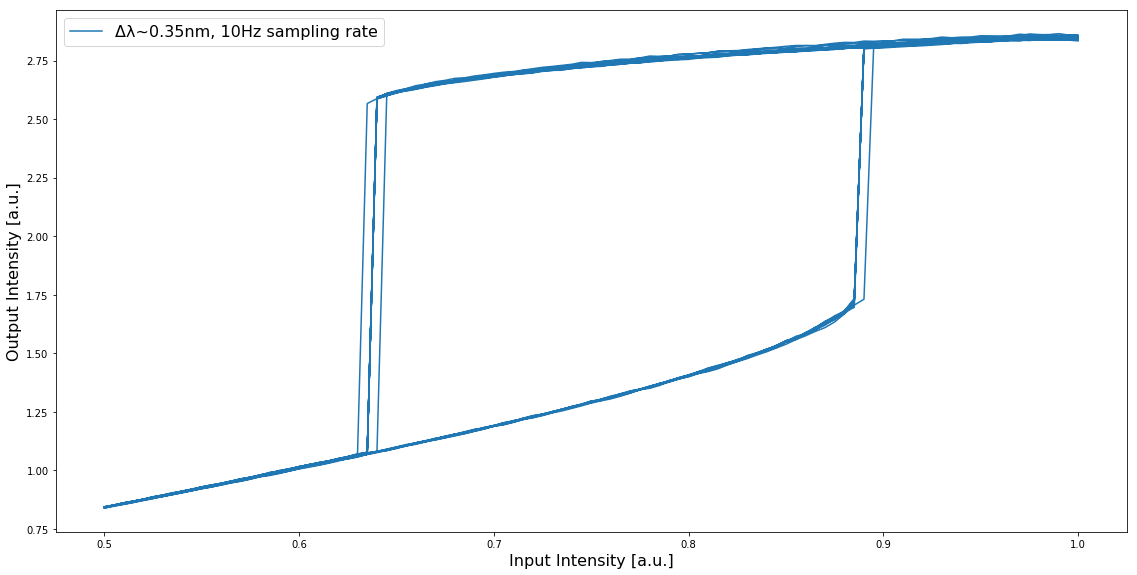
\includegraphics[draft,width=9cm,height=6cm]{figures/foo.png}
	\caption{image/scheme of the conv NN}
	\label{fig:convolutionalNN}
\end{figure}


\subsection{Other Types of NNs}
\label{ssec:Other_Types_of_NNs}
By changing the topology of the nodes distribution and their connections, one obtain other networks that cannot be catalogued under the class of feedforward networks.
Moreover, those different types of network are not a niche, but are widely \ref{} studied as a different approach to the same or additional problems.

\subsubsection{Recurrent NN}
\label{sssec:Recurrent_NN}
Recurrent neural network are a kind of network in which a portion of the input of nodes depends on the (past) output of the same nodes or nodes of subsequent layers.
That is information does not propagates only forward like in the feedforward networks, but can propagate also backward, for example in loops or in feedbacks.

\subsubsection{Reservoir NN}
\label{sssec:Reservoir_NN}
Reservoir neural networks differ from feedforward and recurrent networks in the learning approach.
In fact, the topology of a reservoir network could be exactly the same as that of a deep multi-layer perceptron or that of a recurrent network.
However, the reservoir computing approach claims that it is not necessary to learn all the weights of the network, but only for the last (perceptron) layer.

\begin{figure}[ht]
	\centering
	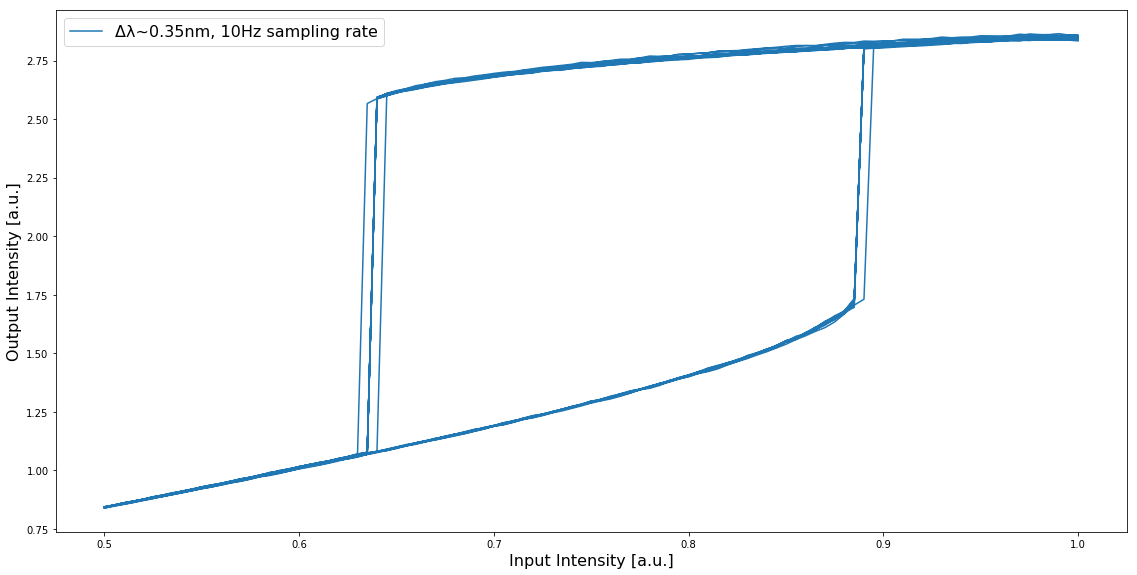
\includegraphics[draft,width=9cm,height=6cm]{figures/foo.png}
	\caption{image/scheme of the reservoir NN}
	\label{fig:reservoirNN}
\end{figure}

These kind of networks, then, can be trained much faster than their respective counterparts, i.e. feedforward and recurrent,
\subsubsection{Modular NN}
\label{sec:Modular_NN}


\subsubsection{Spiking NN}
\label{sec:Spiking_NN}
Spiking artificial networks are the most different kind in respect to all the other networks until now described.
In this class of ANNs, information is not coded only in the intensity of the signal, but also in the rate of signals, e.g. a high value will be encoded as a signal with high repetition rate, whereas a low value as a signal with low repetition rate.
This way of encoding information is more alike the mechanism of biological neural networks, such as our brain \ref{}.

\vspace{1em}
\noindent LOOK INTO other type of neuron model: Hodgkin–Huxley (H-H) model
\url{ https://en.wikipedia.org/wiki/Binding_neuron }

\section{Real-Life Examples}
\label{sec:Real-Life_Examples}
\noindent\uppercase{\large{? Should I keep this section ?}}
\normalsize

\section{ANN Simulation}
\label{sec:ANN_Simulation}
The resources and the time available allowed me to implement physically only the activation function of one node.
Hence, to test this hardware implementation as I will show in \autoref{sec:Test_of_a_Trained ANN} of \autoref{ch:experiments}, I had first to simulate and train \textit{offline} a specific neural network.
To do so, I chose a programming language, \textit{Python}, and a library, \textit{PyTorch}, which helped me in this task.
\subsection{PyTorch}
\label{PyTorch}

PyTorch is a python package that provides high-level features such as a deep learning research platform \cite{PyTorch.org}.
It is based on a backpropagation algorithm called \textit{Reverse-mode auto-differentiation}, which is fast and flexible.
Moreover integrates acceleration libraries that allow fast and lean operation.

To summarize, the library was chosen for its language and its flexibility, even though it is also powerful.
This because our need was to simulate a little network to test the activation function.